% Options for packages loaded elsewhere
\PassOptionsToPackage{unicode}{hyperref}
\PassOptionsToPackage{hyphens}{url}
%
\documentclass[
]{article}
\usepackage{amsmath,amssymb}
\usepackage{iftex}
\ifPDFTeX
  \usepackage[T1]{fontenc}
  \usepackage[utf8]{inputenc}
  \usepackage{textcomp} % provide euro and other symbols
\else % if luatex or xetex
  \usepackage{unicode-math} % this also loads fontspec
  \defaultfontfeatures{Scale=MatchLowercase}
  \defaultfontfeatures[\rmfamily]{Ligatures=TeX,Scale=1}
\fi
\usepackage{lmodern}
\ifPDFTeX\else
  % xetex/luatex font selection
\fi
% Use upquote if available, for straight quotes in verbatim environments
\IfFileExists{upquote.sty}{\usepackage{upquote}}{}
\IfFileExists{microtype.sty}{% use microtype if available
  \usepackage[]{microtype}
  \UseMicrotypeSet[protrusion]{basicmath} % disable protrusion for tt fonts
}{}
\makeatletter
\@ifundefined{KOMAClassName}{% if non-KOMA class
  \IfFileExists{parskip.sty}{%
    \usepackage{parskip}
  }{% else
    \setlength{\parindent}{0pt}
    \setlength{\parskip}{6pt plus 2pt minus 1pt}}
}{% if KOMA class
  \KOMAoptions{parskip=half}}
\makeatother
\usepackage{xcolor}
\usepackage[margin=1in]{geometry}
\usepackage{color}
\usepackage{fancyvrb}
\newcommand{\VerbBar}{|}
\newcommand{\VERB}{\Verb[commandchars=\\\{\}]}
\DefineVerbatimEnvironment{Highlighting}{Verbatim}{commandchars=\\\{\}}
% Add ',fontsize=\small' for more characters per line
\usepackage{framed}
\definecolor{shadecolor}{RGB}{248,248,248}
\newenvironment{Shaded}{\begin{snugshade}}{\end{snugshade}}
\newcommand{\AlertTok}[1]{\textcolor[rgb]{0.94,0.16,0.16}{#1}}
\newcommand{\AnnotationTok}[1]{\textcolor[rgb]{0.56,0.35,0.01}{\textbf{\textit{#1}}}}
\newcommand{\AttributeTok}[1]{\textcolor[rgb]{0.13,0.29,0.53}{#1}}
\newcommand{\BaseNTok}[1]{\textcolor[rgb]{0.00,0.00,0.81}{#1}}
\newcommand{\BuiltInTok}[1]{#1}
\newcommand{\CharTok}[1]{\textcolor[rgb]{0.31,0.60,0.02}{#1}}
\newcommand{\CommentTok}[1]{\textcolor[rgb]{0.56,0.35,0.01}{\textit{#1}}}
\newcommand{\CommentVarTok}[1]{\textcolor[rgb]{0.56,0.35,0.01}{\textbf{\textit{#1}}}}
\newcommand{\ConstantTok}[1]{\textcolor[rgb]{0.56,0.35,0.01}{#1}}
\newcommand{\ControlFlowTok}[1]{\textcolor[rgb]{0.13,0.29,0.53}{\textbf{#1}}}
\newcommand{\DataTypeTok}[1]{\textcolor[rgb]{0.13,0.29,0.53}{#1}}
\newcommand{\DecValTok}[1]{\textcolor[rgb]{0.00,0.00,0.81}{#1}}
\newcommand{\DocumentationTok}[1]{\textcolor[rgb]{0.56,0.35,0.01}{\textbf{\textit{#1}}}}
\newcommand{\ErrorTok}[1]{\textcolor[rgb]{0.64,0.00,0.00}{\textbf{#1}}}
\newcommand{\ExtensionTok}[1]{#1}
\newcommand{\FloatTok}[1]{\textcolor[rgb]{0.00,0.00,0.81}{#1}}
\newcommand{\FunctionTok}[1]{\textcolor[rgb]{0.13,0.29,0.53}{\textbf{#1}}}
\newcommand{\ImportTok}[1]{#1}
\newcommand{\InformationTok}[1]{\textcolor[rgb]{0.56,0.35,0.01}{\textbf{\textit{#1}}}}
\newcommand{\KeywordTok}[1]{\textcolor[rgb]{0.13,0.29,0.53}{\textbf{#1}}}
\newcommand{\NormalTok}[1]{#1}
\newcommand{\OperatorTok}[1]{\textcolor[rgb]{0.81,0.36,0.00}{\textbf{#1}}}
\newcommand{\OtherTok}[1]{\textcolor[rgb]{0.56,0.35,0.01}{#1}}
\newcommand{\PreprocessorTok}[1]{\textcolor[rgb]{0.56,0.35,0.01}{\textit{#1}}}
\newcommand{\RegionMarkerTok}[1]{#1}
\newcommand{\SpecialCharTok}[1]{\textcolor[rgb]{0.81,0.36,0.00}{\textbf{#1}}}
\newcommand{\SpecialStringTok}[1]{\textcolor[rgb]{0.31,0.60,0.02}{#1}}
\newcommand{\StringTok}[1]{\textcolor[rgb]{0.31,0.60,0.02}{#1}}
\newcommand{\VariableTok}[1]{\textcolor[rgb]{0.00,0.00,0.00}{#1}}
\newcommand{\VerbatimStringTok}[1]{\textcolor[rgb]{0.31,0.60,0.02}{#1}}
\newcommand{\WarningTok}[1]{\textcolor[rgb]{0.56,0.35,0.01}{\textbf{\textit{#1}}}}
\usepackage{longtable,booktabs,array}
\usepackage{calc} % for calculating minipage widths
% Correct order of tables after \paragraph or \subparagraph
\usepackage{etoolbox}
\makeatletter
\patchcmd\longtable{\par}{\if@noskipsec\mbox{}\fi\par}{}{}
\makeatother
% Allow footnotes in longtable head/foot
\IfFileExists{footnotehyper.sty}{\usepackage{footnotehyper}}{\usepackage{footnote}}
\makesavenoteenv{longtable}
\usepackage{graphicx}
\makeatletter
\newsavebox\pandoc@box
\newcommand*\pandocbounded[1]{% scales image to fit in text height/width
  \sbox\pandoc@box{#1}%
  \Gscale@div\@tempa{\textheight}{\dimexpr\ht\pandoc@box+\dp\pandoc@box\relax}%
  \Gscale@div\@tempb{\linewidth}{\wd\pandoc@box}%
  \ifdim\@tempb\p@<\@tempa\p@\let\@tempa\@tempb\fi% select the smaller of both
  \ifdim\@tempa\p@<\p@\scalebox{\@tempa}{\usebox\pandoc@box}%
  \else\usebox{\pandoc@box}%
  \fi%
}
% Set default figure placement to htbp
\def\fps@figure{htbp}
\makeatother
\setlength{\emergencystretch}{3em} % prevent overfull lines
\providecommand{\tightlist}{%
  \setlength{\itemsep}{0pt}\setlength{\parskip}{0pt}}
\setcounter{secnumdepth}{-\maxdimen} % remove section numbering
\usepackage{booktabs}
\usepackage{longtable}
\usepackage{array}
\usepackage{multirow}
\usepackage{wrapfig}
\usepackage{float}
\usepackage{colortbl}
\usepackage{pdflscape}
\usepackage{tabu}
\usepackage{threeparttable}
\usepackage{threeparttablex}
\usepackage[normalem]{ulem}
\usepackage{makecell}
\usepackage{xcolor}
\usepackage{bookmark}
\IfFileExists{xurl.sty}{\usepackage{xurl}}{} % add URL line breaks if available
\urlstyle{same}
\hypersetup{
  pdftitle={Predict heart disease based on certain Health factors},
  pdfauthor={Anjal Hussan},
  hidelinks,
  pdfcreator={LaTeX via pandoc}}

\title{Predict heart disease based on certain Health factors}
\author{Anjal Hussan}
\date{July 29, 2024}

\begin{document}
\maketitle

{
\setcounter{tocdepth}{4}
\tableofcontents
}
\newpage

\section{Abstract}\label{abstract}

For this project we will be using different predictive modeling
techniques that we have learned throughout the course and using real
world data in order to predict if a person has heart disease based on
certain factors. The data set for this project
\href{https://www.kaggle.com/fedesoriano/heart-failure-prediction}{Heart
Failure Prediction Dataset} can be found on Kaggle. Each observation in
this dataset represents a person's health history, including their age,
sex, cholesterol levels, etc. The dataset includes a total of 918
distinct individuals gathered from different countries and agencies.
This dataset includes 12 different features, of categorical and/or
continous values, of an individual health record, including if the
individual has heart disease or not.

\section{Background}\label{background}

Cardiovascular diseases is the number 1 cause of death globally. The WHO
records show that cardiovascular diseases accounted for 31\% of all
deaths worldwide in 2016. According to the CDC, nearly 6.2 million
adults in the United States suffer heart failure, and in 2018 alone,
heart failure was mentioned on 379,800 death certificates. Also, the
treatment cost of health care services and medicines is costly and
estimated about 31 billion in 2012. Early detection and management for
heart disease could be effective in reducing the incidence of heart
failure.

Note that heart failure occurs when the heart cannot pump enough blood
and oxygen to support other organs in the body. With this data set, we
would like to see if we can develop a good model to predict if a person
has heart disease and what factors can be attributed to heart disease
most directly. We will be tackling this question with the usage of
different regression techniques and algorithms learned from this class.

\section{Introduction}\label{introduction}

The reason why we have chosen this data set to work with is because of
how relevant this data set is towards the real world. Heart disease is a
condition which affects everyone and being able to successfully predict
heart failure ahead of time can save millions of lives. Data scientist
are studying everyday trying to understand the predictors of heart
failure which is why data sets like this are often on Kaggle in order to
gather data scientist from all over to help solve this issue in order to
help society.

\section{Literature Review}\label{literature-review}

Several papers have been written about heard heart failure detection
using different statistical methodologies - especially related to
classification using machine learning techniques.

An initial search in Google scholar site under
\url{https://scholar.google.com/scholar?hl=en&as_sdt=0\%2C33&q=diagnosis+of+heart+disease&btnG=&oq=diagnosis+of+hear}
returns around 4min paper! Just in 2021, google accounts for 80k papers
and citations.

Given the depth of this study field, we decided to cite one paper that
uses a similar dataset but uses prediction techniques not learned in
this class: Prediction of heart disease and classifiers' sensitivity
analysis by Khaled Mohamad Almustafa published at BMC Bioinformatics
volume 21, Article number: 278 (2020):
\url{https://bmcbioinformatics.biomedcentral.com/articles/10.1186/s12859-020-03626-y\#Abs1}\\
This paper also offers an ample reference of other related paper that
could be beneficial for future related work in this area.

In the paper, a comparative analysis of different classifiers was
performed for the classification of the Heart Disease dataset in order
to correctly classify and or predict HD cases with minimal attributes.
The algorithms used K- Nearest Neighbor (K-NN), Naive Bayes, Decision
tree J48, JRip, SVM, Adaboost, Stochastic Gradient Decent (SGD) and
Decision Table (DT) classifiers to show the performance of the selected
classifications algorithms to best classify, and or predict, the HD
cases.

Result is that using different classification algorithms for the
classification of the HD data set gives very promising results in term
of the classification accuracy for the K-NN (K=1), Decision tree J48 and
JRip classifiers with accuracy of classification of 99.7073, 98.0488 and
97.2683\% respectively.

Main conclusion is to have a reliable feature selection method for HD
disease prediction with using minimal number of attributes instead of
having to consider all available ones.

\section{Methodolgy}\label{methodolgy}

Methodology will follows a typical data science project: from
understanding the dataset through exploratory data analysis, data
preparation, model buildings and finally model evaluation. We seek to
build a model that predicts heart disease, a binary outcome. Prior to
loading and analyzing our data, below, we describe the attributes of the
dataset. This dataset is pulled from a popular Kaggle aggregation and
represents 12 attributes across a sample of males and females from the
age of 28 to 77. Each observation/row in this dataset represents a
person's health records, which include their Age, Sex, ChestPainType,
RestingBP, Cholesterol, FastingBS, RestingECG, MaxHR, ExerciseAngina,
Oldpeak, ST\_Slope, and Heart Disease Status. The dataset is an
aggregation of data from Cleveland, Hungary, Switzerland, Long Beach,
VA, and Stalog and in total, there are 1190 different observations. The
dataset also includes 272 duplicated observations which need to be
removed prior to doing any modeling work. We will also need to clean the
dataset and remove any outliers in the data preparation stage.

In the following analysis, we employ various methods learned in this
class such as a mix combination of statistical analysis, feature
importance selection, and logistic regression modeling and prediction in
order to predict if a person has heart disease or not.

It's common for real-world datasets to contain missing values for
various reasons. They often read as NaN and blank records. These missing
values can significantly alter the machine learning model's quality. One
way to treat these records is to eliminate the observations with missing
data. Unfortunately, we run the risk of losing data points with useful
information. While our dataset does not have \emph{missing values}, per
se, we do encounter zero values that are not intuitive. We deal with
these values through reasonable techniques that enable us to avoid
eliminating records with important data. We'll detail these techniques
below. Further, our final predictive model assigns a \emph{Heart
Disease} positive flag to records wherein the model predicts a
likelihood of greater than 50\%. We determined this to be an appropriate
threshold, but it was a choice, and we understand that predictive health
models might demand a lower threshold for actually providing patients
with health warnings.

\section{Data Exploration}\label{data-exploration}

\subsection{Attribute Information}\label{attribute-information}

\textbf{Age}: age of the patient {[}years{]}\\
\textbf{Sex}: sex of the patient {[}M: Male, F: Female{]}\\
\textbf{ChestPainType}: chest pain type {[}TA: Typical Angina, ATA:
Atypical Angina, NAP: Non-Anginal Pain, ASY: Asymptomatic{]}\\
\textbf{RestingBP}: resting blood pressure {[}mm Hg{]}\\
\textbf{Cholesterol}: serum cholesterol {[}mm/dl{]}\\
\textbf{FastingBS}: fasting blood sugar {[}1: if FastingBS
\textgreater{} 120 mg/dl, 0: otherwise{]}\\
\textbf{RestingECG}: resting electrocardiogram results {[}Normal:
Normal, ST: having ST-T wave abnormality (T wave inversions and/or ST
elevation or depression of \textgreater{} 0.05 mV), LVH: showing
probable or definite left ventricular hypertrophy by Estes'
criteria{]}\\
\textbf{MaxHR}: maximum heart rate achieved {[}Numeric value between 60
and 202{]}\\
\textbf{ExerciseAngina}: exercise-induced angina {[}Y: Yes, N: No{]}\\
\textbf{Oldpeak}: oldpeak = ST {[}Numeric value measured in
depression{]}\\
\textbf{ST\_Slope}: the slope of the peak exercise ST segment {[}Up:
upsloping, Flat: flat, Down: downsloping{]}\\
\textbf{HeartDisease}: output class {[}1: heart disease, 0: Normal{]}

\subsection{Split Dataset}\label{split-dataset}

We split the dataset by allocating 70\% of the dataset to the training
set and 30\% to the test set. The training set will be used to build
models and the evaluation set will be used to evaluate the performance
of the models.

This dataset contain 918 observations and 12 variables. There are 6
integer variables, 5 character variables, and 1 numeric variable.

The response variable will be the \textbf{HeartDisease} and the rest of
11 variables are all predictors.

\begin{verbatim}
## 'data.frame':    918 obs. of  12 variables:
##  $ Age           : int  40 49 37 48 54 39 45 54 37 48 ...
##  $ Sex           : chr  "M" "F" "M" "F" ...
##  $ ChestPainType : chr  "ATA" "NAP" "ATA" "ASY" ...
##  $ RestingBP     : int  140 160 130 138 150 120 130 110 140 120 ...
##  $ Cholesterol   : int  289 180 283 214 195 339 237 208 207 284 ...
##  $ FastingBS     : int  0 0 0 0 0 0 0 0 0 0 ...
##  $ RestingECG    : chr  "Normal" "Normal" "ST" "Normal" ...
##  $ MaxHR         : int  172 156 98 108 122 170 170 142 130 120 ...
##  $ ExerciseAngina: chr  "N" "N" "N" "Y" ...
##  $ Oldpeak       : num  0 1 0 1.5 0 0 0 0 1.5 0 ...
##  $ ST_Slope      : chr  "Up" "Flat" "Up" "Flat" ...
##  $ HeartDisease  : int  0 1 0 1 0 0 0 0 1 0 ...
\end{verbatim}

Below we'll display a few basic EDA techniques to gain insight into our
heart failure dataset.

\subsection{Summary Statistic}\label{summary-statistic}

We can see from quite a few of variables are high variance and skewed.
Also, there are no missing data in this dataset.

\begin{verbatim}
##              vars   n   mean     sd median trimmed   mad  min   max range  skew
## Age             1 918  53.51   9.43   54.0   53.71 10.38 28.0  77.0  49.0 -0.20
## RestingBP       2 918 132.40  18.51  130.0  131.50 14.83  0.0 200.0 200.0  0.18
## Cholesterol     3 918 198.80 109.38  223.0  204.41 68.20  0.0 603.0 603.0 -0.61
## FastingBS       4 918   0.23   0.42    0.0    0.17  0.00  0.0   1.0   1.0  1.26
## MaxHR           5 918 136.81  25.46  138.0  137.23 26.69 60.0 202.0 142.0 -0.14
## Oldpeak         6 918   0.89   1.07    0.6    0.74  0.89 -2.6   6.2   8.8  1.02
## HeartDisease    7 918   0.55   0.50    1.0    0.57  0.00  0.0   1.0   1.0 -0.21
##              kurtosis   se
## Age             -0.40 0.31
## RestingBP        3.23 0.61
## Cholesterol      0.10 3.61
## FastingBS       -0.41 0.01
## MaxHR           -0.46 0.84
## Oldpeak          1.18 0.04
## HeartDisease    -1.96 0.02
\end{verbatim}

\pandocbounded{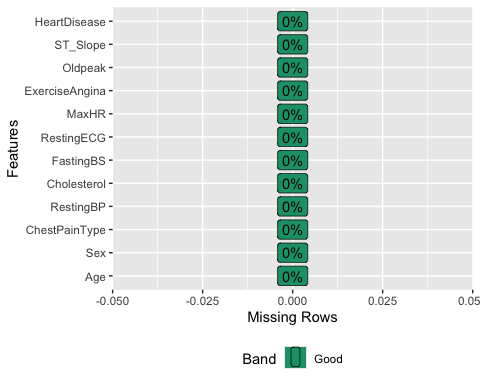
\includegraphics[keepaspectratio]{Predict-Cardiovascular-diseases_files/figure-latex/unnamed-chunk-4-1.pdf}}

From below histogram and density plots, we notice that there are some
zero values for Cholesterol variable. As Cholesterol measurement cannot
be zero, we may need to want to consider replace with mean or median or
impute the zeros.

\pandocbounded{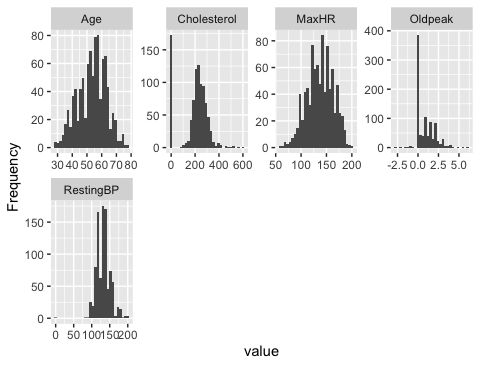
\includegraphics[keepaspectratio]{Predict-Cardiovascular-diseases_files/figure-latex/unnamed-chunk-5-1.pdf}}
\pandocbounded{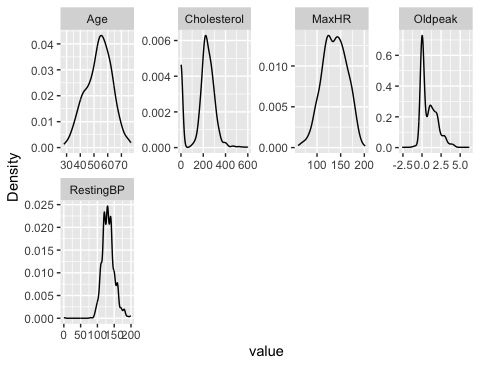
\includegraphics[keepaspectratio]{Predict-Cardiovascular-diseases_files/figure-latex/unnamed-chunk-5-2.pdf}}

For predictors which are character data type, we do count for
categorical for which having heart disease. From below bar plots, we can
notice Male is more likely to get heart disease than women. Also, most
heart disease patients do not feel chest pain, normal blood pressure,
having exercise-induced angina, and flat st segment.

\pandocbounded{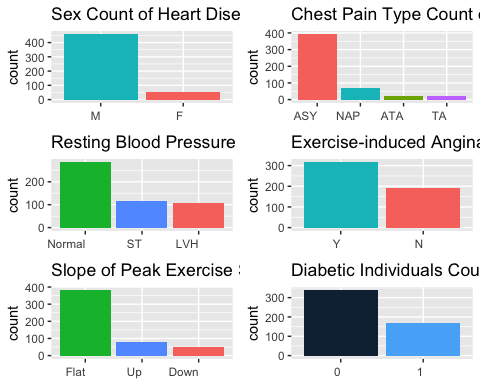
\includegraphics[keepaspectratio]{Predict-Cardiovascular-diseases_files/figure-latex/unnamed-chunk-6-1.pdf}}

\subsection{Identifying
Multicollinearity}\label{identifying-multicollinearity}

The correlation chart below shows some correlation among predictors. We
can do a correlation test for each continuous predictor by using the
Pearson method and at 95\% confidence level to determine if any
correlation among predictors is significant.

\pandocbounded{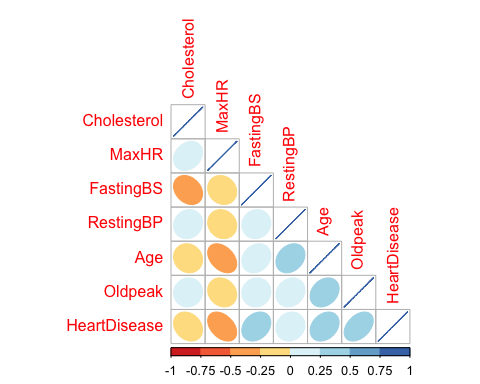
\includegraphics[keepaspectratio]{Predict-Cardiovascular-diseases_files/figure-latex/unnamed-chunk-7-1.pdf}}
From the table below, we can see most pairwise combinations' p-value are
less than 5\% significant level. This indicates those pairwise
combinations are significantly correlated. Note that the effect of
collinearity on prediction is less serious. The accuracy of the
prediction depends on the distance from the observed data. Collinear
data only covers very small fraction of the the predictor space.

\begin{verbatim}
## # A tibble: 30 x 3
##    var1        var2              p
##    <chr>       <chr>         <dbl>
##  1 Cholesterol Oldpeak     0.129  
##  2 Oldpeak     Cholesterol 0.129  
##  3 FastingBS   Oldpeak     0.111  
##  4 Oldpeak     FastingBS   0.111  
##  5 FastingBS   RestingBP   0.0335 
##  6 RestingBP   FastingBS   0.0335 
##  7 Cholesterol Age         0.00386
##  8 Age         Cholesterol 0.00386
##  9 Cholesterol RestingBP   0.00221
## 10 RestingBP   Cholesterol 0.00221
## # i 20 more rows
\end{verbatim}

\section{Data Preparation}\label{data-preparation}

In this section we will be looking at different ways to prepare the data
for modeling and will be showing the different steps and reasons.

To understand the data in a better way, we created the following table
to explain the Definition and the value of each feature.

\begin{longtable}[]{@{}
  >{\raggedright\arraybackslash}p{(\linewidth - 4\tabcolsep) * \real{0.0938}}
  >{\raggedright\arraybackslash}p{(\linewidth - 4\tabcolsep) * \real{0.3188}}
  >{\raggedright\arraybackslash}p{(\linewidth - 4\tabcolsep) * \real{0.5875}}@{}}
\toprule\noalign{}
\begin{minipage}[b]{\linewidth}\raggedright
Feature
\end{minipage} & \begin{minipage}[b]{\linewidth}\raggedright
Definition
\end{minipage} & \begin{minipage}[b]{\linewidth}\raggedright
Value
\end{minipage} \\
\midrule\noalign{}
\endhead
\bottomrule\noalign{}
\endlastfoot
Age & Patient's age in years & 28 - 77 \\
Sex & Gender & (0)female, (1)male \\
ChestPainType & Type of chest-pain & (0)typical angina, (1)atypical
angina, (2)non-angina pain, (3)asymptomatic \\
RestingBP & Resting blood pressure in mmHg & 0 - 200 \\
Cholesterol & Serum cholestoral in mg/dl & 0 -- 603 \\
FastingBS & Fasting blood sugar higher than 120 mg/dl & (0)False
(1)True \\
RestingECG & Resting electrocardiographic results & (0)normal, (1)having
ST-T wave abnormality, (2)showing probable left ventricular
hypertrophy \\
MaxHR & Maximum heart rate achieved & 60 --202 \\
ExerciseAngina & Exercise induced angina & (0)No(1)Yes \\
Oldpeak & ST depression induced by exercise relative to rest & -2.6 -
6.2 \\
ST\_Slope & The slope of the peak exercise ST segment & (1)upsloping,
(2)flat, (3)downsloping \\
HeartDisease & Diagnosis of heart disease & (0)heart disease not
present, (1)heart disease present \\
\end{longtable}

\begin{Shaded}
\begin{Highlighting}[]
\FunctionTok{str}\NormalTok{(train\_data)}
\end{Highlighting}
\end{Shaded}

\begin{verbatim}
## 'data.frame':    643 obs. of  12 variables:
##  $ Age           : int  49 54 39 54 48 37 39 49 54 60 ...
##  $ Sex           : chr  "F" "M" "M" "M" ...
##  $ ChestPainType : chr  "NAP" "NAP" "NAP" "ATA" ...
##  $ RestingBP     : int  160 150 120 110 120 130 120 140 120 100 ...
##  $ Cholesterol   : int  180 195 339 208 284 211 204 234 273 248 ...
##  $ FastingBS     : int  0 0 0 0 0 0 0 0 0 0 ...
##  $ RestingECG    : chr  "Normal" "Normal" "Normal" "Normal" ...
##  $ MaxHR         : int  156 122 170 142 120 142 145 140 150 125 ...
##  $ ExerciseAngina: chr  "N" "N" "N" "N" ...
##  $ Oldpeak       : num  1 0 0 0 0 0 0 1 1.5 1 ...
##  $ ST_Slope      : chr  "Flat" "Up" "Up" "Up" ...
##  $ HeartDisease  : int  1 0 0 0 0 0 0 1 0 1 ...
\end{verbatim}

The `str' function describes the structure of the data. We need to
change/convert most of the features.

\begin{Shaded}
\begin{Highlighting}[]
\CommentTok{\#Change values to 0 and 1}
\CommentTok{\#Sex}
\NormalTok{train\_data}\SpecialCharTok{$}\NormalTok{Sex}\OtherTok{\textless{}{-}}\FunctionTok{ifelse}\NormalTok{(train\_data}\SpecialCharTok{$}\NormalTok{Sex}\SpecialCharTok{==}\StringTok{"M"}\NormalTok{,}\DecValTok{1}\NormalTok{,}\DecValTok{0}\NormalTok{)}
\NormalTok{eval\_data}\SpecialCharTok{$}\NormalTok{Sex}\OtherTok{\textless{}{-}}\FunctionTok{ifelse}\NormalTok{(eval\_data}\SpecialCharTok{$}\NormalTok{Sex}\SpecialCharTok{==}\StringTok{"M"}\NormalTok{, }\DecValTok{1}\NormalTok{, }\DecValTok{0}\NormalTok{)}

\CommentTok{\#ExerciseAngina}
\NormalTok{train\_data}\SpecialCharTok{$}\NormalTok{ExerciseAngina }\OtherTok{\textless{}{-}} \FunctionTok{ifelse}\NormalTok{(train\_data}\SpecialCharTok{$}\NormalTok{ExerciseAngina }\SpecialCharTok{==} \StringTok{"Y"}\NormalTok{, }\DecValTok{1}\NormalTok{,}\DecValTok{0}\NormalTok{)}
\NormalTok{eval\_data}\SpecialCharTok{$}\NormalTok{ExerciseAngina }\OtherTok{\textless{}{-}} \FunctionTok{ifelse}\NormalTok{(eval\_data}\SpecialCharTok{$}\NormalTok{ExerciseAngina }\SpecialCharTok{==} \StringTok{"Y"}\NormalTok{, }\DecValTok{1}\NormalTok{, }\DecValTok{0}\NormalTok{)}
\end{Highlighting}
\end{Shaded}

\begin{Shaded}
\begin{Highlighting}[]
\CommentTok{\#ChestPainType: Change typical angina (TA) to 0, atypical angina (ATA) }
\CommentTok{\#to 1, non{-}angina pain(NAP) to 2, asymptomatic(ASY) to 3.}
\NormalTok{train\_data}\SpecialCharTok{$}\NormalTok{ChestPainType }\OtherTok{=} \FunctionTok{factor}\NormalTok{(train\_data}\SpecialCharTok{$}\NormalTok{ChestPainType, }\AttributeTok{levels =} \FunctionTok{c}\NormalTok{(}\StringTok{\textquotesingle{}TA\textquotesingle{}}\NormalTok{,}\StringTok{\textquotesingle{}ATA\textquotesingle{}}\NormalTok{,}\StringTok{\textquotesingle{}NAP\textquotesingle{}}\NormalTok{,}\StringTok{\textquotesingle{}ASY\textquotesingle{}}\NormalTok{),}
                                  \AttributeTok{labels =} \FunctionTok{c}\NormalTok{(}\StringTok{\textquotesingle{}0\textquotesingle{}}\NormalTok{,}\StringTok{\textquotesingle{}1\textquotesingle{}}\NormalTok{,}\StringTok{\textquotesingle{}2\textquotesingle{}}\NormalTok{,}\StringTok{\textquotesingle{}3\textquotesingle{}}\NormalTok{))}
\NormalTok{eval\_data}\SpecialCharTok{$}\NormalTok{ChestPainType }\OtherTok{=} \FunctionTok{factor}\NormalTok{(eval\_data}\SpecialCharTok{$}\NormalTok{ChestPainType, }\AttributeTok{levels =} \FunctionTok{c}\NormalTok{(}\StringTok{\textquotesingle{}TA\textquotesingle{}}\NormalTok{,}\StringTok{\textquotesingle{}ATA\textquotesingle{}}\NormalTok{,}\StringTok{\textquotesingle{}NAP\textquotesingle{}}\NormalTok{,}\StringTok{\textquotesingle{}ASY\textquotesingle{}}\NormalTok{),}
                                 \AttributeTok{labels =} \FunctionTok{c}\NormalTok{(}\StringTok{\textquotesingle{}0\textquotesingle{}}\NormalTok{,}\StringTok{\textquotesingle{}1\textquotesingle{}}\NormalTok{,}\StringTok{\textquotesingle{}2\textquotesingle{}}\NormalTok{,}\StringTok{\textquotesingle{}3\textquotesingle{}}\NormalTok{))}

\CommentTok{\#RestingECG: 0 for Normal, 1 for ST, and 2 for LVH}
\NormalTok{train\_data}\SpecialCharTok{$}\NormalTok{RestingECG }\OtherTok{=} \FunctionTok{factor}\NormalTok{(train\_data}\SpecialCharTok{$}\NormalTok{RestingECG, }\AttributeTok{levels =} \FunctionTok{c}\NormalTok{(}\StringTok{\textquotesingle{}Normal\textquotesingle{}}\NormalTok{,}\StringTok{\textquotesingle{}ST\textquotesingle{}}\NormalTok{,}\StringTok{\textquotesingle{}LVH\textquotesingle{}}\NormalTok{), }
                               \AttributeTok{labels =} \FunctionTok{c}\NormalTok{(}\StringTok{\textquotesingle{}0\textquotesingle{}}\NormalTok{,}\StringTok{\textquotesingle{}1\textquotesingle{}}\NormalTok{,}\StringTok{\textquotesingle{}2\textquotesingle{}}\NormalTok{))}

\CommentTok{\#ST\_Slope: 0 for UP, 1 for FLAT, and 2 for DOWN}
\NormalTok{train\_data}\SpecialCharTok{$}\NormalTok{ST\_Slope }\OtherTok{=} \FunctionTok{factor}\NormalTok{(train\_data}\SpecialCharTok{$}\NormalTok{ST\_Slope, }\AttributeTok{levels =} \FunctionTok{c}\NormalTok{(}\StringTok{\textquotesingle{}Up\textquotesingle{}}\NormalTok{,}\StringTok{\textquotesingle{}Flat\textquotesingle{}}\NormalTok{,}\StringTok{\textquotesingle{}Down\textquotesingle{}}\NormalTok{), }
                             \AttributeTok{labels =} \FunctionTok{c}\NormalTok{(}\StringTok{\textquotesingle{}0\textquotesingle{}}\NormalTok{,}\StringTok{\textquotesingle{}1\textquotesingle{}}\NormalTok{,}\StringTok{\textquotesingle{}2\textquotesingle{}}\NormalTok{))}

\NormalTok{eval\_data}\SpecialCharTok{$}\NormalTok{RestingECG }\OtherTok{=} \FunctionTok{factor}\NormalTok{(eval\_data}\SpecialCharTok{$}\NormalTok{RestingECG, }\AttributeTok{levels =} \FunctionTok{c}\NormalTok{(}\StringTok{\textquotesingle{}Normal\textquotesingle{}}\NormalTok{,}\StringTok{\textquotesingle{}ST\textquotesingle{}}\NormalTok{,}\StringTok{\textquotesingle{}LVH\textquotesingle{}}\NormalTok{), }
                              \AttributeTok{labels =} \FunctionTok{c}\NormalTok{(}\StringTok{\textquotesingle{}0\textquotesingle{}}\NormalTok{,}\StringTok{\textquotesingle{}1\textquotesingle{}}\NormalTok{,}\StringTok{\textquotesingle{}2\textquotesingle{}}\NormalTok{))}
\CommentTok{\#ST\_Slope: 0 for UP, 1 for FLAT, and 2 for DOWN}
\NormalTok{eval\_data}\SpecialCharTok{$}\NormalTok{ST\_Slope }\OtherTok{=} \FunctionTok{factor}\NormalTok{(eval\_data}\SpecialCharTok{$}\NormalTok{ST\_Slope, }\AttributeTok{levels =} \FunctionTok{c}\NormalTok{(}\StringTok{\textquotesingle{}Up\textquotesingle{}}\NormalTok{,}\StringTok{\textquotesingle{}Flat\textquotesingle{}}\NormalTok{,}\StringTok{\textquotesingle{}Down\textquotesingle{}}\NormalTok{), }
                            \AttributeTok{labels =} \FunctionTok{c}\NormalTok{(}\StringTok{\textquotesingle{}0\textquotesingle{}}\NormalTok{,}\StringTok{\textquotesingle{}1\textquotesingle{}}\NormalTok{,}\StringTok{\textquotesingle{}2\textquotesingle{}}\NormalTok{))}
\end{Highlighting}
\end{Shaded}

\begin{Shaded}
\begin{Highlighting}[]
\CommentTok{\#Convert columns to factor}
\NormalTok{train\_data}\SpecialCharTok{$}\NormalTok{Sex }\OtherTok{\textless{}{-}} \FunctionTok{as.factor}\NormalTok{(train\_data}\SpecialCharTok{$}\NormalTok{Sex)}
\NormalTok{train\_data}\SpecialCharTok{$}\NormalTok{ExerciseAngina }\OtherTok{\textless{}{-}} \FunctionTok{as.factor}\NormalTok{(train\_data}\SpecialCharTok{$}\NormalTok{ExerciseAngina)}
\NormalTok{train\_data}\SpecialCharTok{$}\NormalTok{FastingBS }\OtherTok{\textless{}{-}} \FunctionTok{as.factor}\NormalTok{(train\_data}\SpecialCharTok{$}\NormalTok{FastingBS)}
\NormalTok{train\_data}\SpecialCharTok{$}\NormalTok{HeartDisease }\OtherTok{\textless{}{-}} \FunctionTok{as.factor}\NormalTok{(train\_data}\SpecialCharTok{$}\NormalTok{HeartDisease)}

\CommentTok{\#Convert columns to num}
\NormalTok{train\_data}\SpecialCharTok{$}\NormalTok{RestingBP }\OtherTok{\textless{}{-}} \FunctionTok{as.numeric}\NormalTok{(train\_data}\SpecialCharTok{$}\NormalTok{RestingBP)}
\NormalTok{train\_data}\SpecialCharTok{$}\NormalTok{Age }\OtherTok{\textless{}{-}} \FunctionTok{as.numeric}\NormalTok{(train\_data}\SpecialCharTok{$}\NormalTok{Age)}
\NormalTok{train\_data}\SpecialCharTok{$}\NormalTok{Cholesterol }\OtherTok{\textless{}{-}} \FunctionTok{as.numeric}\NormalTok{(train\_data}\SpecialCharTok{$}\NormalTok{Cholesterol)}
\NormalTok{train\_data}\SpecialCharTok{$}\NormalTok{MaxHR }\OtherTok{\textless{}{-}} \FunctionTok{as.numeric}\NormalTok{(train\_data}\SpecialCharTok{$}\NormalTok{MaxHR)}

\CommentTok{\#eval}
\CommentTok{\#Convert columns to factor}
\NormalTok{eval\_data}\SpecialCharTok{$}\NormalTok{Sex }\OtherTok{\textless{}{-}} \FunctionTok{as.factor}\NormalTok{(eval\_data}\SpecialCharTok{$}\NormalTok{Sex)}
\NormalTok{eval\_data}\SpecialCharTok{$}\NormalTok{ExerciseAngina }\OtherTok{\textless{}{-}} \FunctionTok{as.factor}\NormalTok{(eval\_data}\SpecialCharTok{$}\NormalTok{ExerciseAngina)}
\NormalTok{eval\_data}\SpecialCharTok{$}\NormalTok{FastingBS }\OtherTok{\textless{}{-}} \FunctionTok{as.factor}\NormalTok{(eval\_data}\SpecialCharTok{$}\NormalTok{FastingBS)}
\NormalTok{eval\_data}\SpecialCharTok{$}\NormalTok{HeartDisease }\OtherTok{\textless{}{-}} \FunctionTok{as.factor}\NormalTok{(eval\_data}\SpecialCharTok{$}\NormalTok{HeartDisease)}
\CommentTok{\#Convert columns to num}
\NormalTok{eval\_data}\SpecialCharTok{$}\NormalTok{RestingBP }\OtherTok{\textless{}{-}} \FunctionTok{as.numeric}\NormalTok{(eval\_data}\SpecialCharTok{$}\NormalTok{RestingBP)}
\NormalTok{eval\_data}\SpecialCharTok{$}\NormalTok{Age }\OtherTok{\textless{}{-}} \FunctionTok{as.numeric}\NormalTok{(eval\_data}\SpecialCharTok{$}\NormalTok{Age)}
\NormalTok{eval\_data}\SpecialCharTok{$}\NormalTok{Cholesterol }\OtherTok{\textless{}{-}} \FunctionTok{as.numeric}\NormalTok{(eval\_data}\SpecialCharTok{$}\NormalTok{Cholesterol)}
\NormalTok{eval\_data}\SpecialCharTok{$}\NormalTok{MaxHR }\OtherTok{\textless{}{-}} \FunctionTok{as.numeric}\NormalTok{(eval\_data}\SpecialCharTok{$}\NormalTok{MaxHR)}
\end{Highlighting}
\end{Shaded}

\subsection{Distribution of Heart
Disease}\label{distribution-of-heart-disease}

Next we will be looking at how many data points do we have where the
client has or does not have heart disease. We would like to make sure
that the dataset is has a balance of people with and without heart
disease in order to create an accurate model.

\begin{Shaded}
\begin{Highlighting}[]
\NormalTok{train\_data }\SpecialCharTok{\%\textgreater{}\%}
  \FunctionTok{count}\NormalTok{(HeartDisease)}
\end{Highlighting}
\end{Shaded}

\begin{verbatim}
##   HeartDisease   n
## 1            0 290
## 2            1 353
\end{verbatim}

As we can see from the result the dataset is also balanced as we have
410 datapoints which dont have heart disease and 508 data points with
heart disease. While the dataset might seem balanced on the surface when
we look further we will see that the dataset is not balanced based on
gender

\subsection{Distribution of Heart Disease among males and
females}\label{distribution-of-heart-disease-among-males-and-females}

\begin{Shaded}
\begin{Highlighting}[]
\FunctionTok{xtabs}\NormalTok{(}\SpecialCharTok{\textasciitilde{}}\NormalTok{ HeartDisease }\SpecialCharTok{+}\NormalTok{ Sex, }\AttributeTok{data=}\NormalTok{ train\_data)}
\end{Highlighting}
\end{Shaded}

\begin{verbatim}
##             Sex
## HeartDisease   0   1
##            0 104 186
##            1  38 315
\end{verbatim}

There are 50 females out of 193 who have diagnosed with heart disease
and 458 males out of 725 were diagnosed with heart disease.

This indicates that 63\% of males in this dataset are diagnosed with
heart disease where is only 26\% of females are diagnosed with heart
disease.

\textbf{We can conclude that males are more diagnosed with heart disease
than females}

\pandocbounded{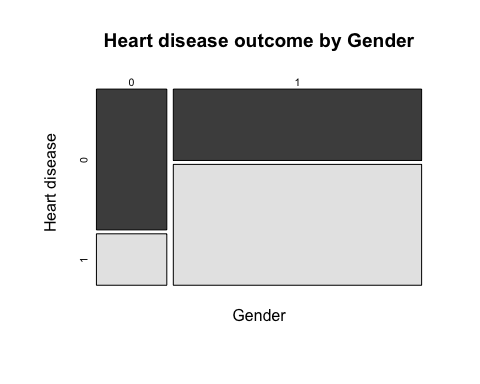
\includegraphics[keepaspectratio]{Predict-Cardiovascular-diseases_files/figure-latex/unnamed-chunk-16-1.pdf}}

\textbf{Numerical Variables}

\pandocbounded{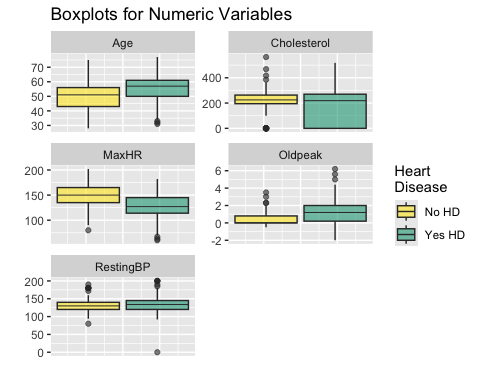
\includegraphics[keepaspectratio]{Predict-Cardiovascular-diseases_files/figure-latex/unnamed-chunk-18-1.pdf}}

\textbf{Categorical Variables}

\pandocbounded{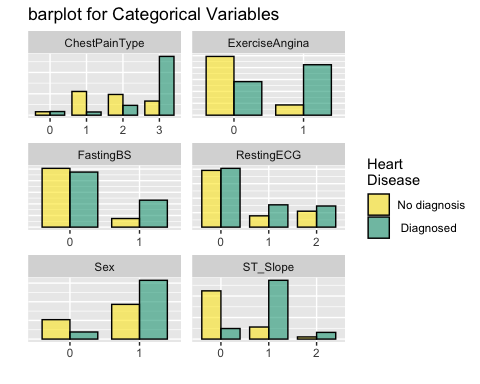
\includegraphics[keepaspectratio]{Predict-Cardiovascular-diseases_files/figure-latex/unnamed-chunk-20-1.pdf}}

\subsection{Missing Data}\label{missing-data}

This dataset seems to not have any missing data which is quite rare for
a dataset. This means that there is not going to be a need to remove the
NA rows or to replace the NA items with the median or mean. But while
the dataset may not have any missing data there might be other issues
that needs to be addressed

\begin{verbatim}
##                na_count
## Age                   0
## Sex                   0
## ChestPainType         0
## RestingBP             0
## Cholesterol           0
## FastingBS             0
## RestingECG            0
## MaxHR                 0
## ExerciseAngina        0
## Oldpeak               0
## ST_Slope              0
## HeartDisease          0
\end{verbatim}

\begin{verbatim}
##                eval_na_count
## Age                        0
## Sex                        0
## ChestPainType              0
## RestingBP                  0
## Cholesterol                0
## FastingBS                  0
## RestingECG                 0
## MaxHR                      0
## ExerciseAngina             0
## Oldpeak                    0
## ST_Slope                   0
## HeartDisease               0
\end{verbatim}

\subsection{Duplicate Row}\label{duplicate-row}

We will be wanting to remove all duplicate rows in the data set in order
to make sure that we will not be skewing results when creating the model

It seems like that our dataset does not have any duplicates as we have
the same amount of rows that we started with.

\subsection{Outliers}\label{outliers}

As seen in the data exploration part of the section we can see that we
have a lot of data values with 0 for \textbf{Cholesterol} and one data
point with 0 \textbf{Resting BP}. As we know it is imposible for humans
to have 0 \textbf{Cholesterol} or 0 \textbf{Resting BP} so we will be
needing to fix this in the dataset. We will be using the median to fix
all the zero values as the median is less susceptible to Outliers. We
will compare results with a dataset where 0 values were excluded from
the set.

\subsubsection{Cholesterol}\label{cholesterol}

Minimun values is now:

\begin{verbatim}
## [1] 100
\end{verbatim}

\subsubsection{Resting BP}\label{resting-bp}

Minimun values is now:

\begin{verbatim}
## [1] 80
\end{verbatim}

\section{Model Creation}\label{model-creation}

We can group the features in four different categories: - Physical
attributes: \emph{age}; \emph{sex} - General Health: \emph{restingBP};
\emph{Cholesterol}; \emph{FastingBS} - ECG related results:
\emph{RestingECG}; \emph{MaxHR}; \emph{Oldpeak}; \emph{ST\_Slope}; -
Symptomatic: \emph{ChestPainType}; \emph{ExerciseAngina}

Considering that the response variable is binary, we start with a
logistic regression with all features included - this is our base model.
We also run the same model on the smaller dataset where 0 values were
excluded from the set.

\begin{Shaded}
\begin{Highlighting}[]
\NormalTok{model1}\OtherTok{\textless{}{-}}\FunctionTok{glm}\NormalTok{(HeartDisease}\SpecialCharTok{\textasciitilde{}}\NormalTok{. , }\AttributeTok{family=}\FunctionTok{binomial}\NormalTok{(}\AttributeTok{link=}\StringTok{"logit"}\NormalTok{), }\AttributeTok{data=}\NormalTok{train\_data)}
\FunctionTok{summary}\NormalTok{(model1)}
\end{Highlighting}
\end{Shaded}

\begin{verbatim}
## 
## Call:
## glm(formula = HeartDisease ~ ., family = binomial(link = "logit"), 
##     data = train_data)
## 
## Coefficients:
##                  Estimate Std. Error z value Pr(>|z|)    
## (Intercept)     -3.573974   1.775540  -2.013 0.044126 *  
## Age              0.017083   0.016012   1.067 0.286039    
## Sex1             1.664790   0.326074   5.106 3.30e-07 ***
## ChestPainType1  -0.851077   0.581390  -1.464 0.143230    
## ChestPainType2  -0.663254   0.521955  -1.271 0.203832    
## ChestPainType3   1.133861   0.508903   2.228 0.025877 *  
## RestingBP        0.001837   0.007309   0.251 0.801554    
## Cholesterol      0.002765   0.002466   1.121 0.262234    
## FastingBS1       1.123248   0.314313   3.574 0.000352 ***
## RestingECG1     -0.028971   0.368037  -0.079 0.937257    
## RestingECG2     -0.050650   0.318482  -0.159 0.873641    
## MaxHR           -0.012056   0.005965  -2.021 0.043265 *  
## ExerciseAngina1  0.353979   0.291712   1.213 0.224957    
## Oldpeak          0.496213   0.143590   3.456 0.000549 ***
## ST_Slope1        2.346493   0.285881   8.208 2.25e-16 ***
## ST_Slope2        0.984964   0.540251   1.823 0.068279 .  
## ---
## Signif. codes:  0 '***' 0.001 '**' 0.01 '*' 0.05 '.' 0.1 ' ' 1
## 
## (Dispersion parameter for binomial family taken to be 1)
## 
##     Null deviance: 885.2  on 642  degrees of freedom
## Residual deviance: 418.1  on 627  degrees of freedom
## AIC: 450.1
## 
## Number of Fisher Scoring iterations: 5
\end{verbatim}

\begin{Shaded}
\begin{Highlighting}[]
\NormalTok{model1a}\OtherTok{\textless{}{-}}\FunctionTok{glm}\NormalTok{(HeartDisease}\SpecialCharTok{\textasciitilde{}}\NormalTok{. , }\AttributeTok{family=}\FunctionTok{binomial}\NormalTok{(}\AttributeTok{link=}\StringTok{"logit"}\NormalTok{), }\AttributeTok{data=}\NormalTok{train\_data1)}
\end{Highlighting}
\end{Shaded}

It's surprising to see that neither `cholesterol', `age' nor `blood
pressure' have any significance in the base model. We calculate the
variance inflation factor (VIF) to check for multicollinearity - no
evidence is found thereof.

\begin{Shaded}
\begin{Highlighting}[]
\FunctionTok{vif}\NormalTok{(model1)}
\end{Highlighting}
\end{Shaded}

\begin{verbatim}
##                    GVIF Df GVIF^(1/(2*Df))
## Age            1.281081  1        1.131848
## Sex            1.121009  1        1.058777
## ChestPainType  1.232756  3        1.035491
## RestingBP      1.140338  1        1.067866
## Cholesterol    1.059390  1        1.029267
## FastingBS      1.105947  1        1.051640
## RestingECG     1.183115  2        1.042934
## MaxHR          1.304039  1        1.141945
## ExerciseAngina 1.255460  1        1.120473
## Oldpeak        1.270721  1        1.127263
## ST_Slope       1.397991  2        1.087367
\end{verbatim}

Removing non-significant terms with the help of function `drop1', we fit
a reduced model.

\begin{Shaded}
\begin{Highlighting}[]
\FunctionTok{drop1}\NormalTok{(model1,}\AttributeTok{test=}\StringTok{"Chi"}\NormalTok{)}
\end{Highlighting}
\end{Shaded}

\begin{verbatim}
## Single term deletions
## 
## Model:
## HeartDisease ~ Age + Sex + ChestPainType + RestingBP + Cholesterol + 
##     FastingBS + RestingECG + MaxHR + ExerciseAngina + Oldpeak + 
##     ST_Slope
##                Df Deviance    AIC    LRT  Pr(>Chi)    
## <none>              418.10 450.10                     
## Age             1   419.24 449.24  1.142 0.2852008    
## Sex             1   446.42 476.42 28.317 1.030e-07 ***
## ChestPainType   3   465.30 491.30 47.199 3.153e-10 ***
## RestingBP       1   418.16 448.16  0.063 0.8013920    
## Cholesterol     1   419.37 449.37  1.272 0.2593743    
## FastingBS       1   431.59 461.59 13.492 0.0002396 ***
## RestingECG      2   418.13 446.13  0.027 0.9865795    
## MaxHR           1   422.21 452.21  4.116 0.0424750 *  
## ExerciseAngina  1   419.56 449.56  1.458 0.2271951    
## Oldpeak         1   430.75 460.75 12.653 0.0003749 ***
## ST_Slope        2   494.44 522.44 76.339 < 2.2e-16 ***
## ---
## Signif. codes:  0 '***' 0.001 '**' 0.01 '*' 0.05 '.' 0.1 ' ' 1
\end{verbatim}

\begin{Shaded}
\begin{Highlighting}[]
\NormalTok{model2}\OtherTok{\textless{}{-}}\FunctionTok{glm}\NormalTok{(HeartDisease }\SpecialCharTok{\textasciitilde{}}\NormalTok{ Sex }\SpecialCharTok{+}\NormalTok{ ChestPainType }\SpecialCharTok{+}\NormalTok{ FastingBS }\SpecialCharTok{+}\NormalTok{ MaxHR }\SpecialCharTok{+} 
\NormalTok{              ExerciseAngina }\SpecialCharTok{+}\NormalTok{ Oldpeak }\SpecialCharTok{+}\NormalTok{ ST\_Slope, }
            \AttributeTok{family =} \FunctionTok{binomial}\NormalTok{(}\AttributeTok{link =} \StringTok{"logit"}\NormalTok{), }\AttributeTok{data =}\NormalTok{ train\_data)}
\NormalTok{model2a}\OtherTok{\textless{}{-}}\FunctionTok{glm}\NormalTok{(HeartDisease }\SpecialCharTok{\textasciitilde{}}\NormalTok{ Sex }\SpecialCharTok{+}\NormalTok{ ChestPainType }\SpecialCharTok{+}\NormalTok{ FastingBS }\SpecialCharTok{+}\NormalTok{ MaxHR }\SpecialCharTok{+}
\NormalTok{               ExerciseAngina }\SpecialCharTok{+}\NormalTok{ Oldpeak }\SpecialCharTok{+}\NormalTok{ ST\_Slope, }
             \AttributeTok{family =} \FunctionTok{binomial}\NormalTok{(}\AttributeTok{link =} \StringTok{"logit"}\NormalTok{), }\AttributeTok{data =}\NormalTok{ train\_data1)}

\FunctionTok{summary}\NormalTok{(model2)}
\end{Highlighting}
\end{Shaded}

\begin{verbatim}
## 
## Call:
## glm(formula = HeartDisease ~ Sex + ChestPainType + FastingBS + 
##     MaxHR + ExerciseAngina + Oldpeak + ST_Slope, family = binomial(link = "logit"), 
##     data = train_data)
## 
## Coefficients:
##                  Estimate Std. Error z value Pr(>|z|)    
## (Intercept)     -1.496051   1.020536  -1.466 0.142663    
## Sex1             1.613552   0.319426   5.051 4.39e-07 ***
## ChestPainType1  -0.818665   0.570911  -1.434 0.151583    
## ChestPainType2  -0.634128   0.512480  -1.237 0.215950    
## ChestPainType3   1.157411   0.500307   2.313 0.020701 *  
## FastingBS1       1.173380   0.307695   3.813 0.000137 ***
## MaxHR           -0.014342   0.005501  -2.607 0.009131 ** 
## ExerciseAngina1  0.379072   0.289328   1.310 0.190135    
## Oldpeak          0.534712   0.140731   3.800 0.000145 ***
## ST_Slope1        2.382196   0.283319   8.408  < 2e-16 ***
## ST_Slope2        0.971162   0.529230   1.835 0.066499 .  
## ---
## Signif. codes:  0 '***' 0.001 '**' 0.01 '*' 0.05 '.' 0.1 ' ' 1
## 
## (Dispersion parameter for binomial family taken to be 1)
## 
##     Null deviance: 885.20  on 642  degrees of freedom
## Residual deviance: 420.85  on 632  degrees of freedom
## AIC: 442.85
## 
## Number of Fisher Scoring iterations: 5
\end{verbatim}

Next, we build a model using variables in the physical attributes and
general health groups which are commonly associated with heart diseases:
cholesterol, blood pressure, age and genre. In addition, as related in
the conclusion of the paper cited in the literature review, simple
models seem to perform better.

\begin{Shaded}
\begin{Highlighting}[]
\NormalTok{model3}\OtherTok{\textless{}{-}}\FunctionTok{glm}\NormalTok{(HeartDisease}\SpecialCharTok{\textasciitilde{}}\NormalTok{ Cholesterol }\SpecialCharTok{+}\NormalTok{ Sex }\SpecialCharTok{+}\NormalTok{ RestingBP }\SpecialCharTok{+} 
\NormalTok{              Age }\SpecialCharTok{+}\NormalTok{ FastingBS, }\AttributeTok{family=}\FunctionTok{binomial}\NormalTok{(}\AttributeTok{link=}\StringTok{"logit"}\NormalTok{), }\AttributeTok{data=}\NormalTok{train\_data)}
\NormalTok{model3a}\OtherTok{\textless{}{-}}\FunctionTok{glm}\NormalTok{(HeartDisease}\SpecialCharTok{\textasciitilde{}}\NormalTok{ Cholesterol }\SpecialCharTok{+}\NormalTok{ Sex }\SpecialCharTok{+}\NormalTok{ RestingBP }\SpecialCharTok{+} 
\NormalTok{               Age }\SpecialCharTok{+}\NormalTok{ FastingBS, }\AttributeTok{family=}\FunctionTok{binomial}\NormalTok{(}\AttributeTok{link=}\StringTok{"logit"}\NormalTok{), }\AttributeTok{data=}\NormalTok{train\_data1)}
\FunctionTok{summary}\NormalTok{(model3)}
\end{Highlighting}
\end{Shaded}

\begin{verbatim}
## 
## Call:
## glm(formula = HeartDisease ~ Cholesterol + Sex + RestingBP + 
##     Age + FastingBS, family = binomial(link = "logit"), data = train_data)
## 
## Coefficients:
##              Estimate Std. Error z value Pr(>|z|)    
## (Intercept) -6.869665   0.935400  -7.344 2.07e-13 ***
## Cholesterol  0.005881   0.001829   3.216   0.0013 ** 
## Sex1         1.655573   0.233824   7.080 1.44e-12 ***
## RestingBP    0.007332   0.005086   1.442   0.1494    
## Age          0.059583   0.010620   5.611 2.02e-08 ***
## FastingBS1   0.948904   0.226362   4.192 2.77e-05 ***
## ---
## Signif. codes:  0 '***' 0.001 '**' 0.01 '*' 0.05 '.' 0.1 ' ' 1
## 
## (Dispersion parameter for binomial family taken to be 1)
## 
##     Null deviance: 885.20  on 642  degrees of freedom
## Residual deviance: 737.58  on 637  degrees of freedom
## AIC: 749.58
## 
## Number of Fisher Scoring iterations: 4
\end{verbatim}

We see that `cholesterol' and `age' are now significant when other
variables are excluded. Only `RestingBP' is not significant. We will
then fit a model removing this feature.

\begin{Shaded}
\begin{Highlighting}[]
\NormalTok{model4}\OtherTok{\textless{}{-}}\FunctionTok{glm}\NormalTok{(HeartDisease}\SpecialCharTok{\textasciitilde{}}\NormalTok{ Cholesterol }\SpecialCharTok{+}\NormalTok{ Sex }\SpecialCharTok{+}  
\NormalTok{              Age }\SpecialCharTok{+}\NormalTok{ FastingBS, }\AttributeTok{family=}\FunctionTok{binomial}\NormalTok{(}\AttributeTok{link=}\StringTok{"logit"}\NormalTok{), }\AttributeTok{data=}\NormalTok{train\_data)}
\NormalTok{model4a}\OtherTok{\textless{}{-}}\FunctionTok{glm}\NormalTok{(HeartDisease}\SpecialCharTok{\textasciitilde{}}\NormalTok{ Cholesterol }\SpecialCharTok{+}\NormalTok{ Sex }\SpecialCharTok{+} 
\NormalTok{               Age }\SpecialCharTok{+}\NormalTok{ FastingBS, }\AttributeTok{family=}\FunctionTok{binomial}\NormalTok{(}\AttributeTok{link=}\StringTok{"logit"}\NormalTok{), }\AttributeTok{data=}\NormalTok{train\_data1)}
\FunctionTok{summary}\NormalTok{(model4)}
\end{Highlighting}
\end{Shaded}

\begin{verbatim}
## 
## Call:
## glm(formula = HeartDisease ~ Cholesterol + Sex + Age + FastingBS, 
##     family = binomial(link = "logit"), data = train_data)
## 
## Coefficients:
##              Estimate Std. Error z value Pr(>|z|)    
## (Intercept) -6.113435   0.765394  -7.987 1.38e-15 ***
## Cholesterol  0.005992   0.001827   3.279  0.00104 ** 
## Sex1         1.652323   0.232876   7.095 1.29e-12 ***
## Age          0.063198   0.010355   6.103 1.04e-09 ***
## FastingBS1   0.943187   0.225621   4.180 2.91e-05 ***
## ---
## Signif. codes:  0 '***' 0.001 '**' 0.01 '*' 0.05 '.' 0.1 ' ' 1
## 
## (Dispersion parameter for binomial family taken to be 1)
## 
##     Null deviance: 885.20  on 642  degrees of freedom
## Residual deviance: 739.68  on 638  degrees of freedom
## AIC: 749.68
## 
## Number of Fisher Scoring iterations: 4
\end{verbatim}

Next, we build a model using variables in the other categories: ECG
related results and symptomatic.

\begin{Shaded}
\begin{Highlighting}[]
\NormalTok{model5}\OtherTok{\textless{}{-}}\FunctionTok{glm}\NormalTok{(HeartDisease}\SpecialCharTok{\textasciitilde{}}\NormalTok{  MaxHR }\SpecialCharTok{+}\NormalTok{ RestingECG }\SpecialCharTok{+}\NormalTok{ Oldpeak }\SpecialCharTok{+}\NormalTok{ ST\_Slope}\SpecialCharTok{+}
\NormalTok{              ChestPainType }\SpecialCharTok{+}\NormalTok{ ExerciseAngina, }\AttributeTok{family=}\FunctionTok{binomial}\NormalTok{(}\AttributeTok{link=}\StringTok{"logit"}\NormalTok{), }\AttributeTok{data=}\NormalTok{train\_data)}
\NormalTok{model5a}\OtherTok{\textless{}{-}}\FunctionTok{glm}\NormalTok{(HeartDisease}\SpecialCharTok{\textasciitilde{}}\NormalTok{ MaxHR }\SpecialCharTok{+}\NormalTok{ RestingECG }\SpecialCharTok{+}\NormalTok{ Oldpeak }\SpecialCharTok{+}\NormalTok{ ST\_Slope}\SpecialCharTok{+}
\NormalTok{              ChestPainType }\SpecialCharTok{+}\NormalTok{ ExerciseAngina, }\AttributeTok{family=}\FunctionTok{binomial}\NormalTok{(}\AttributeTok{link=}\StringTok{"logit"}\NormalTok{), }\AttributeTok{data=}\NormalTok{train\_data1)}
\FunctionTok{summary}\NormalTok{(model5)}
\end{Highlighting}
\end{Shaded}

\begin{verbatim}
## 
## Call:
## glm(formula = HeartDisease ~ MaxHR + RestingECG + Oldpeak + ST_Slope + 
##     ChestPainType + ExerciseAngina, family = binomial(link = "logit"), 
##     data = train_data)
## 
## Coefficients:
##                  Estimate Std. Error z value Pr(>|z|)    
## (Intercept)      0.836351   0.892402   0.937 0.348660    
## MaxHR           -0.017566   0.005249  -3.347 0.000818 ***
## RestingECG1      0.359177   0.330597   1.086 0.277280    
## RestingECG2      0.097866   0.294544   0.332 0.739690    
## Oldpeak          0.472785   0.134705   3.510 0.000448 ***
## ST_Slope1        2.236799   0.258598   8.650  < 2e-16 ***
## ST_Slope2        1.295325   0.509862   2.541 0.011068 *  
## ChestPainType1  -1.359014   0.528204  -2.573 0.010085 *  
## ChestPainType2  -0.870118   0.473108  -1.839 0.065893 .  
## ChestPainType3   0.814581   0.457868   1.779 0.075228 .  
## ExerciseAngina1  0.397534   0.278149   1.429 0.152944    
## ---
## Signif. codes:  0 '***' 0.001 '**' 0.01 '*' 0.05 '.' 0.1 ' ' 1
## 
## (Dispersion parameter for binomial family taken to be 1)
## 
##     Null deviance: 885.20  on 642  degrees of freedom
## Residual deviance: 465.38  on 632  degrees of freedom
## AIC: 487.38
## 
## Number of Fisher Scoring iterations: 5
\end{verbatim}

We now fit a reduced model with only significant features.

\begin{Shaded}
\begin{Highlighting}[]
\NormalTok{model6}\OtherTok{\textless{}{-}}\FunctionTok{glm}\NormalTok{(HeartDisease}\SpecialCharTok{\textasciitilde{}}\NormalTok{  MaxHR }\SpecialCharTok{+}\NormalTok{  Oldpeak }\SpecialCharTok{+}\NormalTok{ ST\_Slope}\SpecialCharTok{+}
\NormalTok{              ChestPainType, }\AttributeTok{family=}\FunctionTok{binomial}\NormalTok{(}\AttributeTok{link=}\StringTok{"logit"}\NormalTok{), }\AttributeTok{data=}\NormalTok{train\_data)}
\NormalTok{model6a}\OtherTok{\textless{}{-}}\FunctionTok{glm}\NormalTok{(HeartDisease}\SpecialCharTok{\textasciitilde{}}\NormalTok{ MaxHR }\SpecialCharTok{+}\NormalTok{  Oldpeak }\SpecialCharTok{+}\NormalTok{ ST\_Slope}\SpecialCharTok{+}
\NormalTok{              ChestPainType , }\AttributeTok{family=}\FunctionTok{binomial}\NormalTok{(}\AttributeTok{link=}\StringTok{"logit"}\NormalTok{), }\AttributeTok{data=}\NormalTok{train\_data1)}
\FunctionTok{summary}\NormalTok{(model6)}
\end{Highlighting}
\end{Shaded}

\begin{verbatim}
## 
## Call:
## glm(formula = HeartDisease ~ MaxHR + Oldpeak + ST_Slope + ChestPainType, 
##     family = binomial(link = "logit"), data = train_data)
## 
## Coefficients:
##                 Estimate Std. Error z value Pr(>|z|)    
## (Intercept)     1.238281   0.867795   1.427  0.15360    
## MaxHR          -0.020018   0.005049  -3.964 7.36e-05 ***
## Oldpeak         0.527472   0.131115   4.023 5.75e-05 ***
## ST_Slope1       2.302119   0.253553   9.079  < 2e-16 ***
## ST_Slope2       1.388893   0.503776   2.757  0.00583 ** 
## ChestPainType1 -1.313230   0.527204  -2.491  0.01274 *  
## ChestPainType2 -0.827387   0.472868  -1.750  0.08017 .  
## ChestPainType3  0.933429   0.452517   2.063  0.03914 *  
## ---
## Signif. codes:  0 '***' 0.001 '**' 0.01 '*' 0.05 '.' 0.1 ' ' 1
## 
## (Dispersion parameter for binomial family taken to be 1)
## 
##     Null deviance: 885.20  on 642  degrees of freedom
## Residual deviance: 468.66  on 635  degrees of freedom
## AIC: 484.66
## 
## Number of Fisher Scoring iterations: 5
\end{verbatim}

\section{Model Selection}\label{model-selection}

In order to select a model, we will compare various metrics for all
seven models using the training data set. We'll employ confusion
matrices, accuracy, and other metrics to ensure we're selecting the most
complete, descriptive model.

\pandocbounded{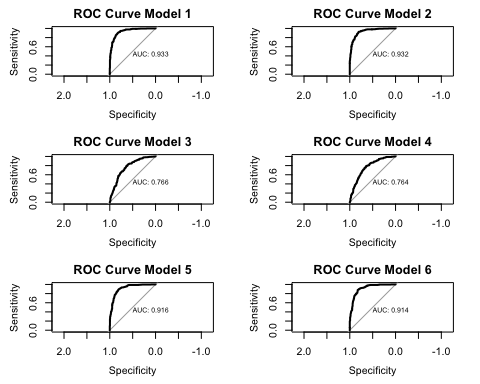
\includegraphics[keepaspectratio]{Predict-Cardiovascular-diseases_files/figure-latex/unnamed-chunk-32-1.pdf}}

\begin{longtabu} to \linewidth {>{\raggedright}X>{\raggedleft}X>{\raggedleft}X>{\raggedleft}X>{\raggedleft}X>{\raggedleft}X>{\raggedleft}X}
\toprule
 & Model 1 & Model 2 & Model 3 & Model 4 & Model 5 & Model 6\\
\midrule
Accuracy & 0.8646967 & 0.8646967 & 0.7216174 & 0.7138414 & 0.8475894 & 0.8538103\\
Class. Error Rate & 0.1353033 & 0.1353033 & 0.2783826 & 0.2861586 & 0.1524106 & 0.1461897\\
Sensitivity & 0.8951841 & 0.8980170 & 0.8101983 & 0.8073654 & 0.8725212 & 0.8838527\\
Specificity & 0.8275862 & 0.8241379 & 0.6137931 & 0.6000000 & 0.8172414 & 0.8172414\\
Precision & 0.8633880 & 0.8614130 & 0.7185930 & 0.7107232 & 0.8531856 & 0.8547945\\
\addlinespace
F1 & 0.8789986 & 0.8793343 & 0.7616511 & 0.7559682 & 0.8627451 & 0.8690808\\
AUC & 0.9333594 & 0.9322555 & 0.7658640 & 0.7641692 & 0.9157273 & 0.9141008\\
MAE & 0.1991055 & 0.2005980 & 0.3892085 & 0.3907681 & 0.2235838 & 0.2258416\\
RMSE & 0.3165007 & 0.3174513 & 0.4401616 & 0.4412094 & 0.3347397 & 0.3366285\\
R2 & 0.5954358 & 0.5929977 & 0.2175769 & 0.2138301 & 0.5474549 & 0.5423363\\
\bottomrule
\end{longtabu}

We now do the same with the alternative modes on the smaller dataset
where 0 values were excluded from the set.

\pandocbounded{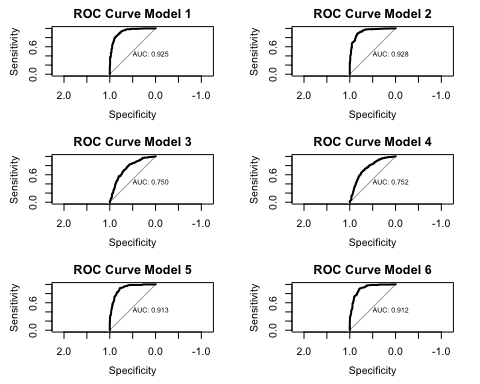
\includegraphics[keepaspectratio]{Predict-Cardiovascular-diseases_files/figure-latex/unnamed-chunk-34-1.pdf}}

\begin{longtabu} to \linewidth {>{\raggedright}X>{\raggedleft}X>{\raggedleft}X>{\raggedleft}X>{\raggedleft}X>{\raggedleft}X>{\raggedleft}X}
\toprule
 & Model 1a & Model 2a & Model 3a & Model 4a & Model 5a & Model 6a\\
\midrule
Accuracy & 0.8699809 & 0.8699809 & 0.6940727 & 0.6978967 & 0.8489484 & 0.8451243\\
Class. Error Rate & 0.1300191 & 0.1300191 & 0.3059273 & 0.3021033 & 0.1510516 & 0.1548757\\
Sensitivity & 0.8795181 & 0.8835341 & 0.6987952 & 0.6947791 & 0.8554217 & 0.8433735\\
Specificity & 0.8613139 & 0.8576642 & 0.6897810 & 0.7007299 & 0.8430657 & 0.8467153\\
Precision & 0.8521401 & 0.8494208 & 0.6718147 & 0.6784314 & 0.8320312 & 0.8333333\\
\addlinespace
F1 & 0.8656126 & 0.8661417 & 0.6850394 & 0.6865079 & 0.8435644 & 0.8383234\\
AUC & 0.9254860 & 0.9280844 & 0.7504591 & 0.7519000 & 0.9129921 & 0.9120885\\
MAE & 0.1868795 & 0.1935835 & 0.3909816 & 0.3959343 & 0.2131376 & 0.2172183\\
RMSE & 0.3071226 & 0.3124255 & 0.4416762 & 0.4444911 & 0.3279149 & 0.3311605\\
R2 & 0.6218586 & 0.6086846 & 0.2179142 & 0.2079130 & 0.5689278 & 0.5603578\\
\bottomrule
\end{longtabu}

The two tables above demonstrates that our first two logistic regression
models provide the most explanatory value. Using the dataset which we
replaced 0 values with the median, our ``kitchen sink'' model enjoys the
highest accuracy and R-squared values while maintaining the lowest MAE
and RMSE values. Finally, its ROC curve makes clear that Model 1 is the
best choice.

Using the dataset which 0 values were excluded from the set, model 2 is
on par with model 1 - our ``kitchen sink'', in most metrics while
displaying a higher AUC. Considering that is always better to choose
parsimonious models, this is the model selected.

\section{Conclusion}\label{conclusion}

We conclude stating that this prediction exercise is very important
because it deals directly with a diseases that is the number 1 cause of
death globally. Although our model accuracy does not get close to 99\%
accuracy as stated in some papers we reviewed, we believe the results
are satisfactory for the purpose of this project.

\end{document}
